\documentclass[a4paper,12pt]{article}

\usepackage[utf8x]{inputenc}
\usepackage[T2A]{fontenc}
\usepackage[english, russian]{babel}

% Опционно, требует  apt-get install scalable-cyrfonts.*
% и удаления одной строчки в cyrtimes.sty
% Сточку не удалять!
% \usepackage{cyrtimes}

% Картнки и tikz
\usepackage{graphicx}
\usepackage{tikz}
\usetikzlibrary{snakes,arrows,shapes}


% Некоторая русификация.
\usepackage{misccorr}
\usepackage{indentfirst}
\renewcommand{\labelitemi}{\normalfont\bfseries{--}}

% Увы, поля придётся уменьшить из-за листингов.
\topmargin -1cm
\oddsidemargin -0.5cm
\evensidemargin -0.5cm
\textwidth 17cm
\textheight 24cm

\sloppy

% Оглавление в PDF
\usepackage[
bookmarks=true,
colorlinks=true, linkcolor=black, anchorcolor=black, citecolor=black, menucolor=black,filecolor=black, urlcolor=black,
unicode=true
]{hyperref}

% Для исходного кода в тексте
\newcommand{\Code}[1]{\texttt{#1}}


\title{Отчёт по лабораторной работе \\ <<Динамическая IP-маршрутизация>>}
\author{(Здесь писать Ф.~И.~О)}

\begin{document}

\maketitle

\tableofcontents

\section{Настройка сети}

\subsection{Топология сети}

Топология сети и используемые IP-адреса показаны на рисунке~\ref{fig:network}.

\begin{figure}
\centering
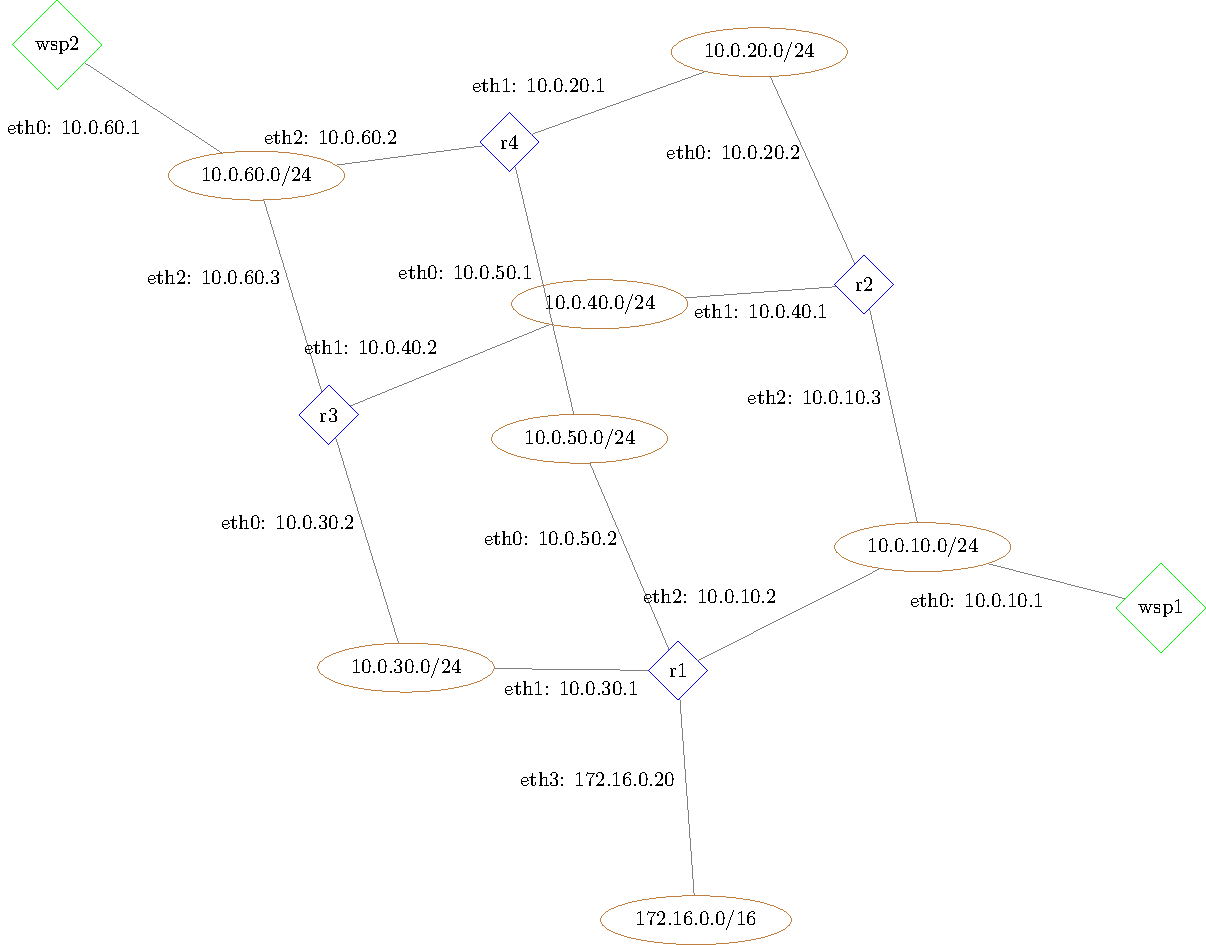
\includegraphics[width=0.8\textwidth]{includes/network_gv.pdf}
\caption{Топология сети}
\label{fig:network}
\end{figure}

Перечень узлов, на которых используется динамическая IP-маршрутизация: ...


\subsection{Назначение IP-адресов}

Ниже приведён файл сетевой настройки  маршрутизатора (указать, какого).

\begin{Verbatim}
Сюда нужно поместить характерный /etc/network/interfaces маршрутизатора
\end{Verbatim}

Ниже приведён файл сетевой настройки рабочей станции (указать, какой).

\begin{Verbatim}
Сюда нужно поместить характерный /etc/network/interfaces рабочей станции
\end{Verbatim}



\subsection{Настройка протокола RIP}

Ниже приведен файл \Code{/etc/quagga/ripd.conf} маршрутизатора (указать, какого).

\begin{Verbatim}
Сюда нужно поместить конфигурацию ripd
\end{Verbatim}


Ниже приведен файл \Code{/etc/quagga/ripd.conf} рабочий станции, связанной с несколькими маршрутизаторами (указать, какой).

\begin{Verbatim}
Сюда нужно поместить конфигурацию ripd
\end{Verbatim}


\section{Проверка настройки протокола RIP}

Вывод \textbf{traceroute} от узла такого-то до такого-то при нормальной работе сети.

\begin{Verbatim}
Сюда нужно поместить вывод traceroute.
\end{Verbatim}

Вывод \textbf{traceroute} от узла такого-то до внешнего IP (195.19.38.2 сгодится).

\begin{Verbatim}
Сюда нужно поместить вывод traceroute.
\end{Verbatim}

Вывод сообщения RIP.

\begin{Verbatim}
Перехваченное сообщение RIP от любого маршрутизатора
\end{Verbatim}

Вывод таблицы RIP.

\begin{Verbatim}
Таблица RIP
\end{Verbatim}

Вывод таблицы маршрутизации.

\begin{Verbatim}
Таблица маршрутизации
\end{Verbatim}

\section{Расщепленный горизонт и испорченные обратные обновления}

Поместить сюда вывод сообщения одного и того же маршрутизатор с включенным расщ. горизонтом, с включенными испорченными обновлениями, с отключённым расщ. гор.

Объяснить разницу.

Вернуть настройки в исходное состояние (включенный без испорченных).

\section{Имитация устранимой поломки в сети}

Какой маршрутизатор выключили?

Вывод таблицы RIP непосредственно перед истечением таймера устаревания (на маршрутизаторе-соседе отключенного).

\begin{Verbatim}
Таблица RIP
\end{Verbatim}

Перестроенная таблица на этом же маршрутизаторе

\begin{Verbatim}
Таблица RIP
\end{Verbatim}


Вывод \textbf{traceroute} от узла такого-то до такого-то после того, как служба RIP перестроила таблицы маршрутизации.

\begin{Verbatim}
Сюда нужно поместить вывод traceroute после "поломки".
\end{Verbatim}

\section{Имитация неустранимой поломки в сети}

Какой маршрутизатор выключили? (Теперь у нас нет связанной сети)

Далее поместить таблицы протокола RIP, где видна 16-ая метрика, и сообщения протокола RIP с 16-ой метрикой.

\end{document}
